\documentclass[../main.tex]{subfiles}
\graphicspath{{figures/}{../figures/}}

\begin{document}
  \todo[color=green!40]{完成问题三模型的建立(sections/q3\_build)}
  \noindent\textbf{Step 1 起始螺距}
  \par   记调头空间半径\(R = 4.5m\)。通过问题二,我们已知在螺距为\(55cm\)时,舞龙队盘入的终止时刻(板凳之间不发生碰撞的最晚时刻即$t_1$)龙头前把手的极径$\rho _0(t_1)$,将两者进行对比可知,\(\rho _0(t_1)<R\) ,这表明在该螺距下,舞龙队能够在不发生碰撞的前提下盘入调头空间。
  \par 因此,将\(55cm\)作为后续搜寻最小螺距的起始上限值,以此为基础逐步缩小螺距范围。
  \\\textbf{Step 2 最小螺距的确定}
  \par 为了搜寻到最小螺距,我们进行以下步骤:
  \\\noindent\textbf{1.初始螺距和步长的确定}
  \par 将\(55cm\)作为初始螺距值,选取\(0.01m\)作为步长开始减小螺距。
  \\\noindent\textbf{2.判断是否发生碰撞}
  \par 在每一轮计算中,首先确定龙头板凳到达调头空间边界的时间\(t\) 。在时间区间\([0, t]\)内,运用问题二中建立的碰撞判断模型,以此精确判断第$i(i=3,\cdots,223)$节板凳与龙头、第\(2\)块板凳之间是否发生碰撞。
  \\\noindent\textbf{3.循环迭代}
  \begin{itemize}
  \item 若在当前螺距下未检测到碰撞,则确定了螺距的上界,以该螺距为初始值,按照设定步长减小螺距,并再次进行碰撞判断;
  \item 若发生碰撞,则确定了螺距的范围,以此螺距为下界,将步长缩小为原来的十分之一(即从\(0.01m\)调整为\(0.001m\) ),在该范围内继续进行碰撞判断.
  \end{itemize}
  \noindent\textbf{4.终止}
  \par 最终,将步长为$10^{-6}$作为循环的终止条件,得到较为精确的满足条件的最小螺距。
  \textbf{Step 3 流程图 }
  \begin{figure}[H]
    \centering
    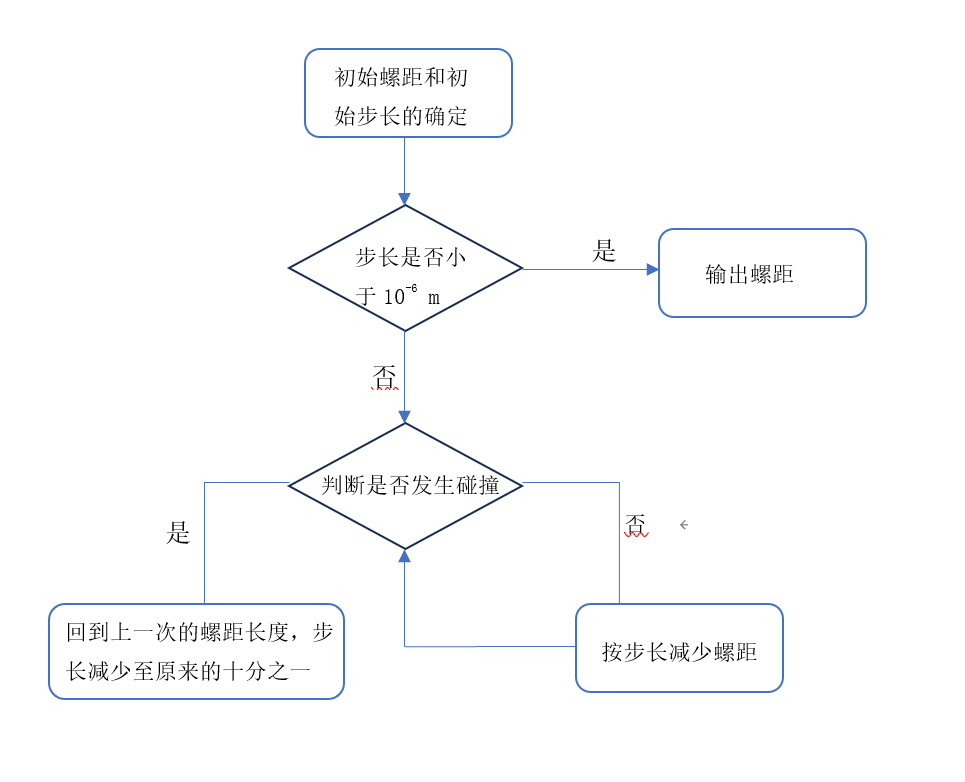
\includegraphics[width=.6\textwidth]{1234}
    \caption{板凳顶点示意图}
    \label{1.1.1.1.1.1.1.1.1.1.1}
\end{figure}

  \end{document}